\section{Systematic Uncertainties}
\label{sec:ewk:syst}

The effect of the systematic uncertainties discussed in Sections \ref{sec:common_syst} and \ref{sec:common_backgrounds} 
is summarized in Figure \ref{fig:syst_etmiss}, which shows the relative size of each group of systematics after the fit in the 
\glspl{cr}. 
The grouping of the systematics is the same as discussed for the gluino search in Section \ref{sec:strong:syst}. 

For what concerns the experimental uncertainties, the largest ones are those on \gls{jes}, 
whose impact on the expected background yields ranges between 5\% and 60\% in the different \glspl{sr}, 
and on the \gls{jer}, which impacts the background yields by 10--50\%. 
The uncertainties on the measured $b$-tagging efficiencies have in general a smaller impact on the background yields, 
which ranges between 10\% and 60\%. 

The largest theoretical uncertainties are the ones on the modeling of the \ttbar background, which range between 10\% and 45\% for the various regions. 
Another uncertainty related to the \ttbar background is the statistical uncertainty due to the finite size of the \gls{cr} samples used to derive  the $\ttbar$ normalization factors, which ranges from 5\% to 25\% and is represented as a separate contribution in Figure \ref{fig:syst_etmiss}.  
The uncertainties on the modeling of the $W/Z$+jets backgrounds  
impact the total yields by 5--20\% in the various regions. 
The modeling uncertainties on the single-top background have a smaller effect on the background yields, leading to changes of at most 11\%. 

The \gls{mc} statistical uncertainty reaches 50\% in SR-4b-meff1-A, but is typically lower, around 20\%. 
 
The total uncertainty, which takes into account correlations between the individual uncertainty sources, ranges between 30\% and 80\% 
of the total background yields in the different regions. 
 

\begin{figure}[htbp]
	\centering
	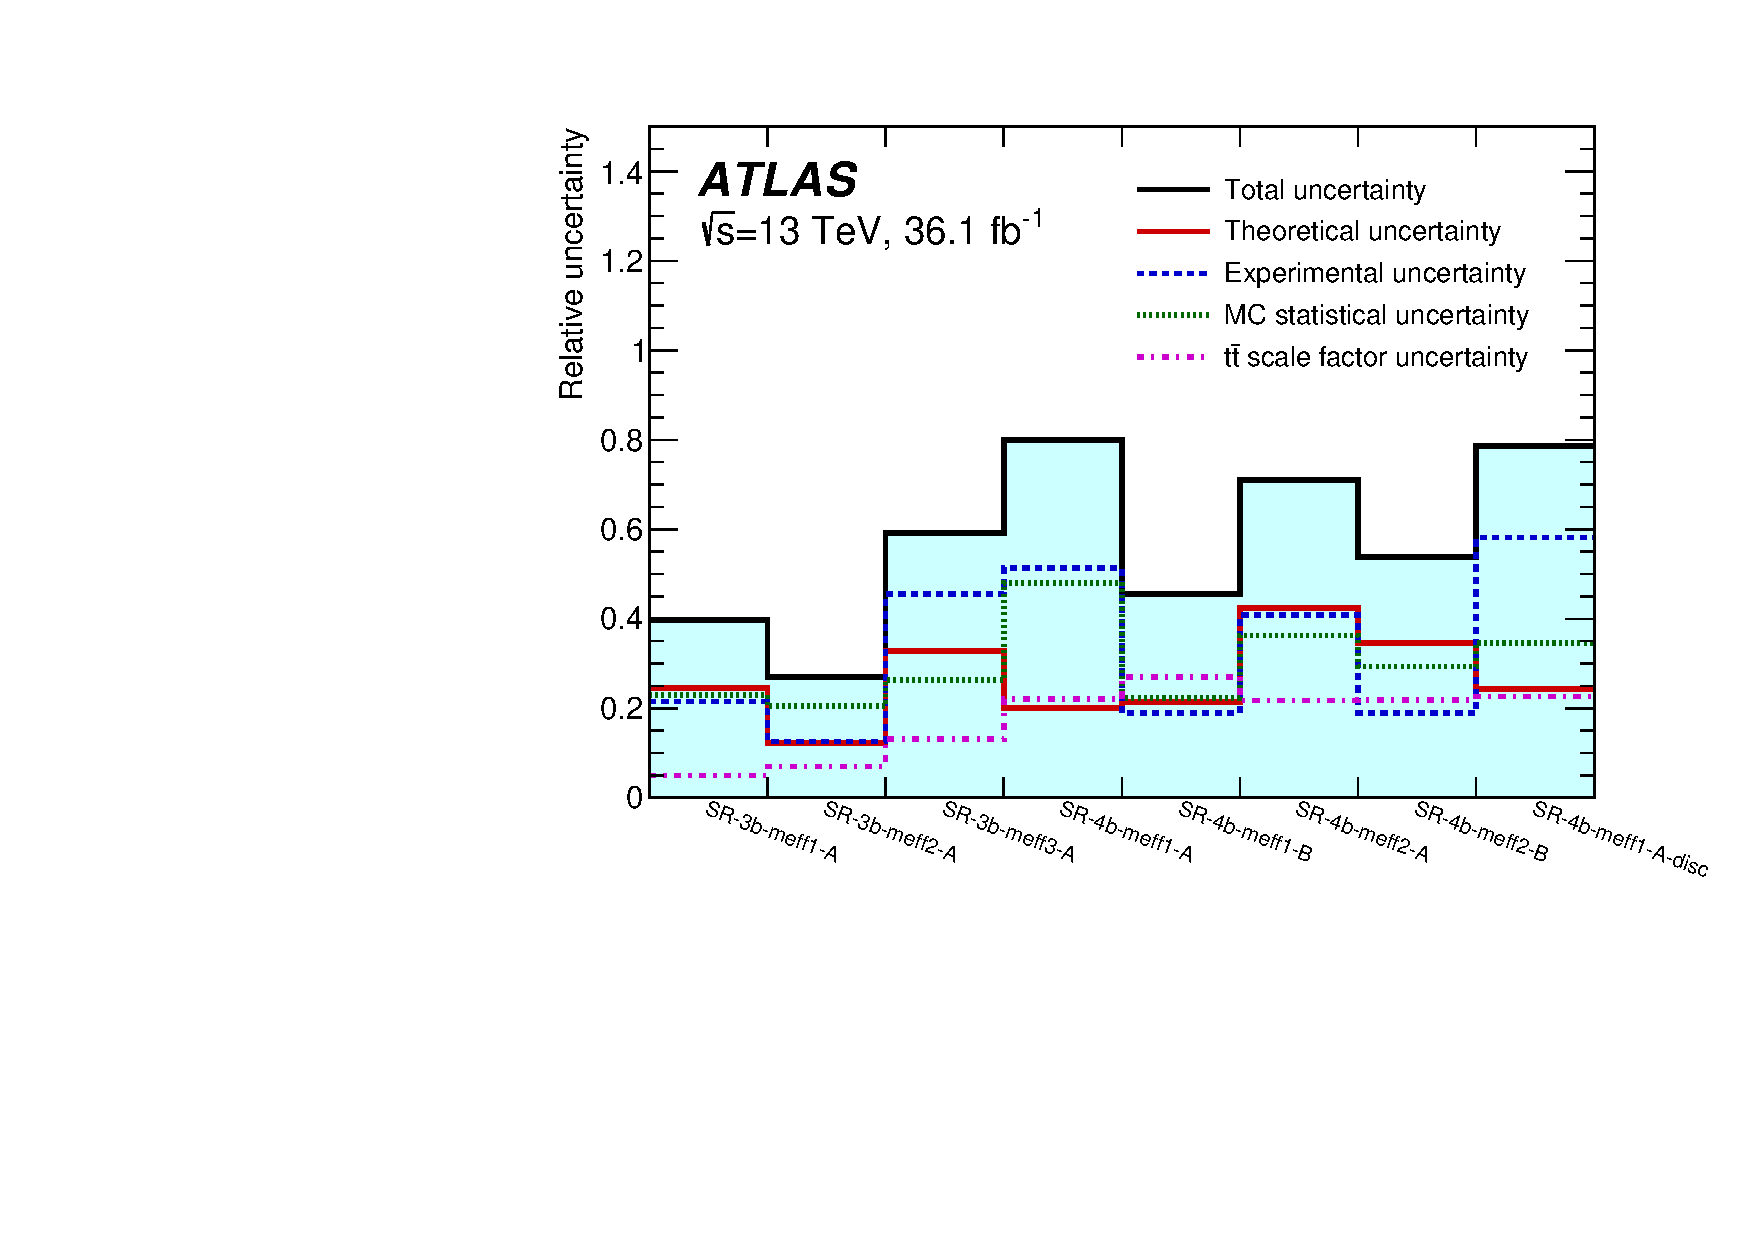
\includegraphics[width=0.85\textwidth]{figures/ewk_prod/etmiss_misc/High-MET-syst.pdf}
	\caption{Relative systematic uncertainties in the background estimate for the high-mass analysis. The individual uncertainties can be correlated, such that the total background uncertainty is not necessarily their sum in quadrature. Figure from Ref. \cite{Aaboud:2018htj}. 
	} 
	\label{fig:syst_etmiss}
\end{figure}

\section{Results}
\label{sec:ewk:results}

Figure \ref{fig:ewk:pullCR} shows the comparison between data and simulation in the \glspl{cr} before the fit (top panel)
and the scale factor for the \ttbar background that is derived from the fit in the \glspl{cr} (bottom panel).
If we compare with the equivalent result for the gluino search, in Figure \ref{fig:pullCR}, it is possible 
to see that on average the \ttbar scale factors have values closer to one. 
This is again because of the improvement in the $b$-tagging calibration of $c$-jets was implemented in this analyses. 
The fit in the \glspl{cr} is extrapolated to the \glspl{vr} and to the \glspl{sr}. 

The post-fit data-\gls{mc} agreement in the \glspl{vr} is shown in Figure \ref{fig:ewk:pullVR}: the top panel of this figure 
shows the post-fit predicted yields in each of the \glspl{vr} and the data yields, while the bottom panel quantifies the 
difference between observed data and predictions in terms of the significance, defined as in Ref. \cite{Choudalakis:2011okv}. 
Note that this is different from the pull definition adopted in the gluino search. 
The closure in the \glspl{vr} is good: all the bins have discrepancies with significance lower than 0.8. 

The results in the \glspl{sr} are shown in Figure \ref{fig:ewk:pullSR}. As in Figure \ref{fig:ewk:pullVR}, the top panel shows the 
predicted and observed yields in each \gls{sr}, and the bottom panel the significance of the discrepancy. 
No significant excess is observed and the observations are in agreement with the \gls{sm} predictions. 
The numerical results of the background-only fit extrapolated to the \glspl{sr} are presented in Table \ref{tab:ewk:yieldsSR},
where the background prediction is also broken down by component. 
This table shows also the total background prediction before the fit in the \glspl{cr}, which is labeled as ``MC-only background''.


\begin{figure}[htbp]
	\centering
	\includegraphics[width=0.9\textwidth]{figures/ewk_prod/etmiss_results/histpull_pulls_in_CR_qcdStrong}
	\caption{Event yields in control regions and related \ttbar\
          normalization factors after the background-only fit for
          %Inputs and results of the likelihood fit in the control
          %regions of
          the high-mass analysis. The upper panel shows 
		the observed number of events and the predicted background yield before the fit.
		All uncertainties  shown in Figure \ref{fig:syst_etmiss} are included in the uncertainty band. The background category $\ttbar+X$ includes $\ttbar W/Z$, $\ttbar H$, and $\ttbar \ttbar$ events.  
		The $\ttbar$ normalization is obtained from the fit
                and is displayed in the bottom panel. Figure from Ref. \cite{Aaboud:2018htj}.
	} 
	\label{fig:ewk:pullCR}
\end{figure}


\begin{figure}[htbp]
	\centering
	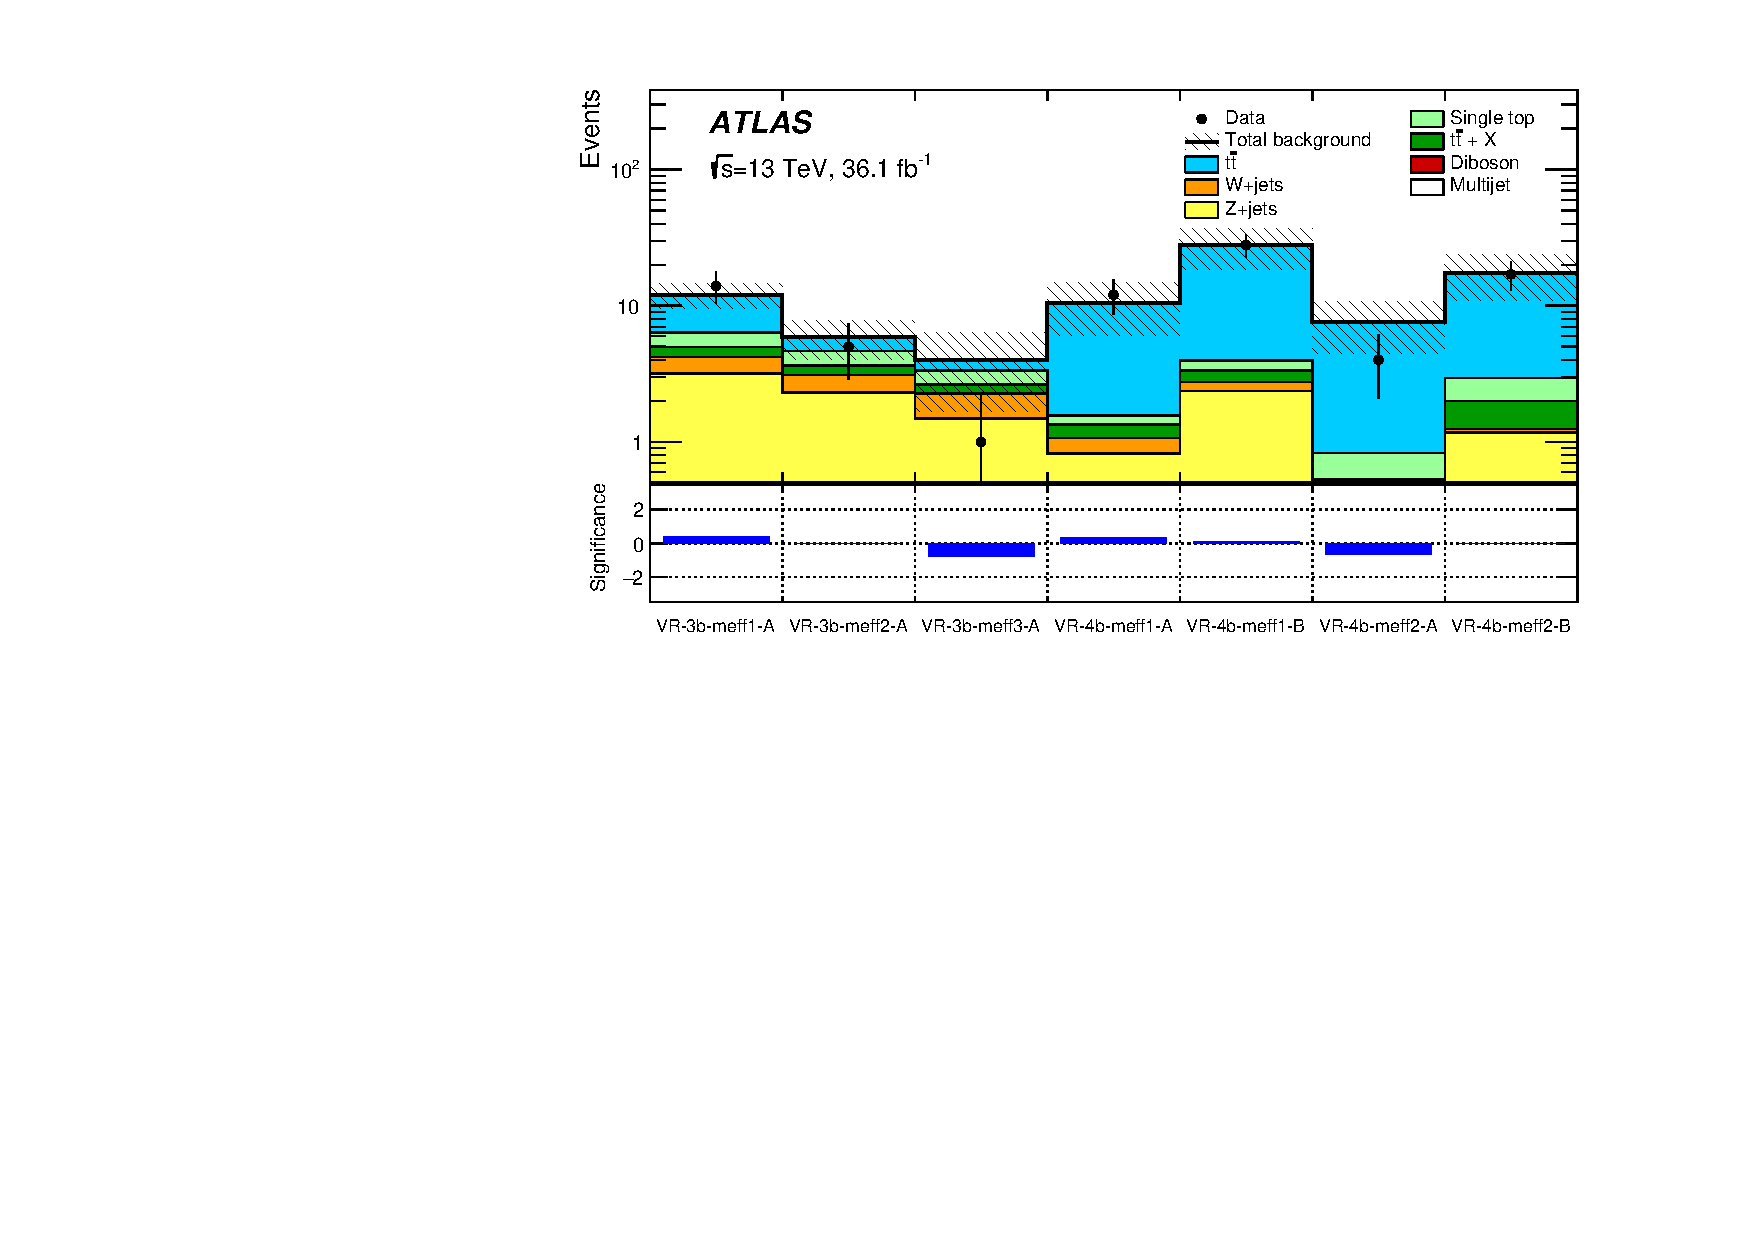
\includegraphics[width=0.9\textwidth]{figures/ewk_prod/etmiss_results/histpull_pulls_in_VR_qcdStrong}
	\caption{Results of the background-only fit extrapolated to the \glspl{vr}. 
	    The $\ttbar$ normalization is obtained from the fit to the \glspl{cr} shown in Figure~\ref{fig:ewk:pullCR}. The upper panel shows 
		the observed number of events and the predicted background yield. The bottom panel shows the significance of any disagreement between the data and the background model, computed as in Ref. \cite{Choudalakis:2011okv}.
		All uncertainties  shown in Figure \ref{fig:syst_etmiss} are included in the 
		uncertainty band. The background category $\ttbar+X$ includes $\ttbar W/Z$, 
		$\ttbar H$, and $\ttbar \ttbar$ events. Figure from Ref. \cite{Aaboud:2018htj}.}
	\label{fig:ewk:pullVR}
\end{figure}

\begin{figure}[htbp]
	\centering
	% \subfigure[]{\includegraphics[width=0.65\textwidth]{figures/etmiss_results/histpull_pulls_in_CR_qcdStrong}\label{fig:pullCR}}\\
	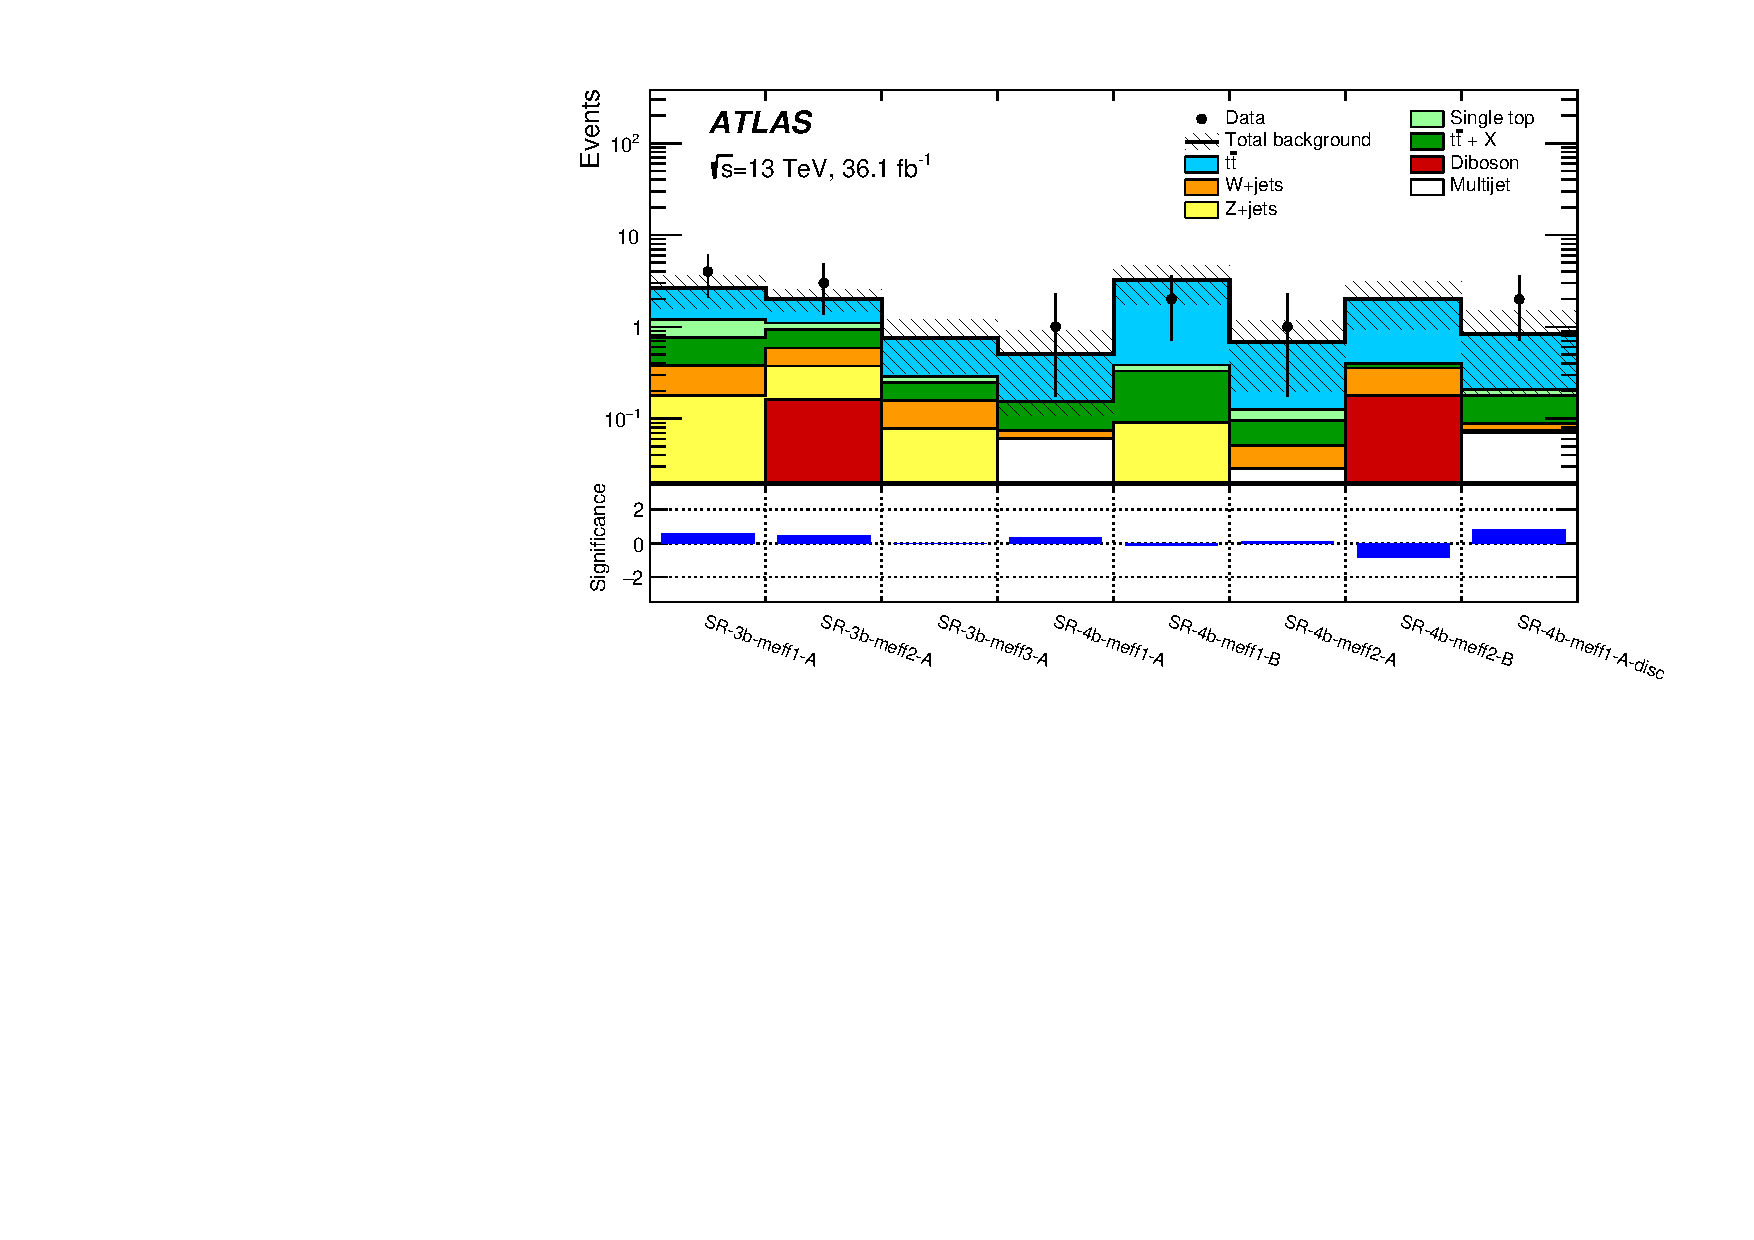
\includegraphics[width=0.9\textwidth]{figures/ewk_prod/etmiss_results/histpull_pulls_in_SR_qcdStrong}
	\caption{Results of the background only fit extrapolated to the \glspl{sr}. 
	The $\ttbar$ normalization is obtained from the fit to the CRs shown in Figure~\ref{fig:pullCR}. The data in the  SRs are 
	not included in the fit.  The upper panel shows the observed number of events and the predicted background 
	yield.  The bottom panel shows the significance of any disagreement between the data and the background model, computed as in Ref. \cite{Choudalakis:2011okv}. All uncertainties  shown in Figure \ref{fig:syst_etmiss} are included in the uncertainty band. 
	The background
	category $\ttbar+X$ includes $\ttbar W/Z$, $\ttbar H$, and $\ttbar \ttbar$ events. Figure from Ref. \cite{Aaboud:2018htj}.} 
	\label{fig:ewk:pullSR}
\end{figure}

\begin{table}
%\resizebox{1.\textwidth}{!}{
\renewcommand{\arraystretch}{1.1}
\begin{tabular}{l|c|c|c|c}
\toprule
SR name & SR-3b-meff1-A & SR-3b-meff2-A & SR-3b-meff3-A & SR-4b-meff1-A \\
\hline
$N_{\mathrm{obs}}$ & 4 & 3 & 0 & 1 \\
\hline
Total background & 2.6 $\pm$ 1.0 & 2.0 $\pm$ 0.5 & 0.8 $\pm$ 0.5 & 0.5 $\pm$ 0.4  \\
Fitted \ttbar & 1.4 $\pm$ 0.8 & 0.89 $\pm$ 0.32 & 0.5 $\pm$ 0.4 & 0.35 $\pm$ 0.33 \\

Single top & 0.43 $\pm$ 0.29 & 0.17 $\pm$ 0.14 & 0.040 $\pm$ 0.017 & $<$ 0.01 \\
$\ttbar+X$ & 0.39 $\pm$ 0.16 & 0.34 $\pm$ 0.14 & 0.09 $\pm$ 0.04 & 0.08 $\pm$ 0.06  \\
$Z$+jets & 0.18 $\pm$ 0.14 & 0.21 $\pm$ 0.16 & 0.07 $\pm$ 0.20 & $<$ 0.01 \\
$W$+jets & 0.20 $\pm$ 0.06 & 0.21 $\pm$ 0.09 & 0.08 $\pm$ 0.06 & 0.013 $\pm$ 0.009  \\
Diboson & $<$ 0.01 & 0.16 $\pm$ 0.11 & $<$ 0.01 & $<$ 0.01 \\
Multijet & $<$ 0.01 & 0.004 $\pm$ 0.005 & 0.004 $\pm$ 0.006 & 0.06 $\pm$ 0.05 \\
\hline
MC-only background & 2.5 $\pm$ 1.0 & 2.0 $\pm$ 0.5 & 0.6 $\pm$ 0.4 & 0.43 $\pm$ 0.31 \\
\bottomrule
\end{tabular}

\vspace{0.4cm}

\begin{tabular}{l|c|c|c|c}
\toprule
SR name & SR-4b-meff1-B & SR-4b-meff2-A & SR-4b-meff2-B & SR-4b-meff1-A-disc\\
\hline
$N_{\mathrm{obs}}$ & 2 & 1 & 0 & 2\\
\hline
Total background &  3.2 $\pm$ 1.5 & 0.7 $\pm$ 0.5 & 2.0 $\pm$ 1.1 & 0.8 $\pm$ 0.7\\
Fitted \ttbar &  2.8 $\pm$ 1.5 & 0.6 $\pm$ 0.5 & 1.6 $\pm$ 1.0 & 0.6 $\pm$ 0.6\\
Single top &  0.06 $\pm$ 0.13 & 0.030 $\pm$ 0.019 & $<$ 0.01 & 0.030 $\pm$ 0.019\\
$\ttbar+X$ & 0.24 $\pm$ 0.10 & 0.045 $\pm$ 0.025 & 0.039 $\pm$ 0.033 & 0.09 $\pm$ 0.06\\
$Z$+jets &  0.09 $\pm$ 0.04 & $<$ 0.01 & $<$ 0.01 & 0.004 $\pm$ 0.011\\
$W$+jets & $<$ 0.01 & 0.022 $\pm$ 0.027 & 0.18 $\pm$ 0.10 & 0.013 $\pm$ 0.008\\
Diboson &  $<$ 0.01 & $<$ 0.01 & 0.17 $\pm$ 0.08 & $<$ 0.01\\
Multijet &  0.0027 $\pm$ 0.0021 & 0.03 $\pm$ 0.04 & 0.007 $\pm$ 0.012 & 0.07 $\pm$ 0.05\\
\hline
MC-only background & 2.6 $\pm$ 0.9 & 0.43 $\pm$ 0.27 & 1.3 $\pm$ 0.6 & 0.7 $\pm$ 0.5\\
\bottomrule
\end{tabular}
%} 
\caption{Results of the background-only fit extrapolated to the SRs of the high-mass analysis, for the total background prediction and breakdown of the main background sources. 
	The uncertainties shown include all systematic uncertainties. The data in the SRs are not included in the fit. 
	The background category $\ttbar+X$ includes $\ttbar W/Z$, $\ttbar H$, and $\ttbar \ttbar$ events.
	The row ``MC-only background'' provides the total background prediction when the
	$\ttbar$ normalization is obtained from a theoretical
	calculation~\cite{Czakon:2011xx}. Table from Ref. \cite{Aaboud:2018htj}.}
\label{tab:ewk:yieldsSR}
\end{table}




\FloatBarrier

\section{Interpretation}
\label{sec:ewk:interp}

The results presented in Section \ref{sec:ewk:results} are used to set limits on the presence of \gls{bsm} signals.

\subsection{Model-independent limits}
\label{sec:ewk:modelindepUL}

The number of expected and observed events in the two discovery \glspl{sr} SR-4b-meff1-A-disc and SR-3b-meff3-A are used to set model-independent limits on the number of \gls{bsm} events. 
These limits, obtained with the \gls{cls} procedure, ignore any signal contamination in the \glspl{cr} and are reported in Table \ref{tab:ewk:UL_toys}.
In the same table are reported also the model-independent limits obtained from the low-mass analysis, complementary to the analysis 
discussed in this document, which is briefly presented in Section \ref{sec:ewk:LM}. 
To distinguish them from the ones of the low-mass analysis, the results in SR-4b-meff1-A-disc and SR-3b-meff3-A are labeled as 
high-SR-4b-meff1-A-disc and high-SR-3b-meff3-A respectively. 

\begin{table}
\begin{center}
\begin{tabular}{|l|c|c|c|c|c|c|}

%{
%     lr
%      S[table-format=4.1(1)]
%      S[table-format=1.1(2)]
%      S[table-format=2.1(1)]
%      cc
%      }
\toprule
{ Signal channel}           &   $N_\mathrm{obs}$ & $N_\mathrm{pred}$       & $\sigma^\mathrm{95}_\mathrm{vis}$ [fb] &  $S_\mathrm{obs}^\mathrm{95}$  & $S_\mathrm{exp}^\mathrm{95}$ & $p_0$ (Z)  \\
\midrule
high-SR-4b-meff1-A-disc   &    2 &     0.8 $\pm$ 0.7  & 0.15 &   5.5 & ${ 4.2 }^{ +1.3 }_{ -0.4 }$  &  0.15$~$(1.02) \\%
high-SR-3b-meff3-A        &    0 &     0.8 $\pm$ 0.5  & 0.08 &   3.0 & ${ 3.1 }^{ +1.2 }_{ -0.1 }$  &  0.50$~$(0.00) \\%
low-SR-MET0-meff440       & 1063 &    1100 $\pm$ 25   & 2.3  &  56   & ${ 79 }^{ +31 }_{ -23 }$     &  0.50$~$(0.00) \\%
low-SR-MET150-meff440     &   17 &      12 $\pm$ 8    & 0.90 &  22   & ${ 19 }^{ +5 }_{ -4 }$       &  0.21$~$(0.80) \\%
\bottomrule
\end{tabular}
\end{center}
\caption[Model independent upper limits]{For each discovery region, the number of observed events ($N_\mathrm{obs}$), the number of predicted events ($N_\mathrm{pred}$), and 95\% CL upper limits on the visible cross-section ($\sigma^\mathrm{95}_\mathrm{vis}$) and on the number of signal events ($S_\mathrm{obs}^\mathrm{95}$ ) are shown.  The fifth column ($S_\mathrm{exp}^\mathrm{95}$) shows the 95\% CL upper limit on the number of signal events given the expected number (and $\pm 1\sigma$ excursions of the expectation) of background events. The last column indicates the discovery $p$-value ($p(s=0)$) in significance units. The $p$-values are capped at 0.5. Results are obtained with $20\,000$ pseudoexperiments.
Table from Ref. \cite{Aaboud:2018htj}.
}
\label{tab:ewk:UL_toys}
\end{table}

\subsection{Model-dependent limits}
\label{sec:ewk:modeldep}

A combined fit that includes simultaneously all the \glspl{cr} and all the orthogonal \glspl{sr} (i.e. all the \glspl{sr}
except from  SR-4b-meff1-A-disc) is used to place limits on the specific models described in Section \ref{sec:ewk:sig}.

The signal model that is used to optimize the analysis regions is higgsino pair production with \gls{br}$(\hino\rightarrow h \tilde{G})=100$\%.
The 95\% CL upper limit on the total pair production cross-section for this model is shown in Figure \ref{fig:exclusion_high}, 
as a function of \mhino. 
The expected exclusion is between 250 and 830 GeV in \mhino. 
Due to the slight deficit in the region with the highest \meffb selection, the observed exclusion is up to 880 GeV.

A second interpretation of the results is provided in Figure \ref{fig:exclusion_high:BR}, which shows the exclusion contour in the 
plane \gls{br}$(\hino\rightarrow h \tilde{G})$--\mhino, with the assumption \gls{br}$(\hino\rightarrow h \tilde{G})$+\gls{br}$(\hino\rightarrow Z \tilde{G}) =1$.
For $\mhino = 400$ GeV, which is the mass point with the lowest excluded $\sigma/\sigma_{\rm theory}$, we exclude at 95\% \gls{cl}
\glspl{br} as low as 45\%.


\begin{figure}[htbp]
	\centering
	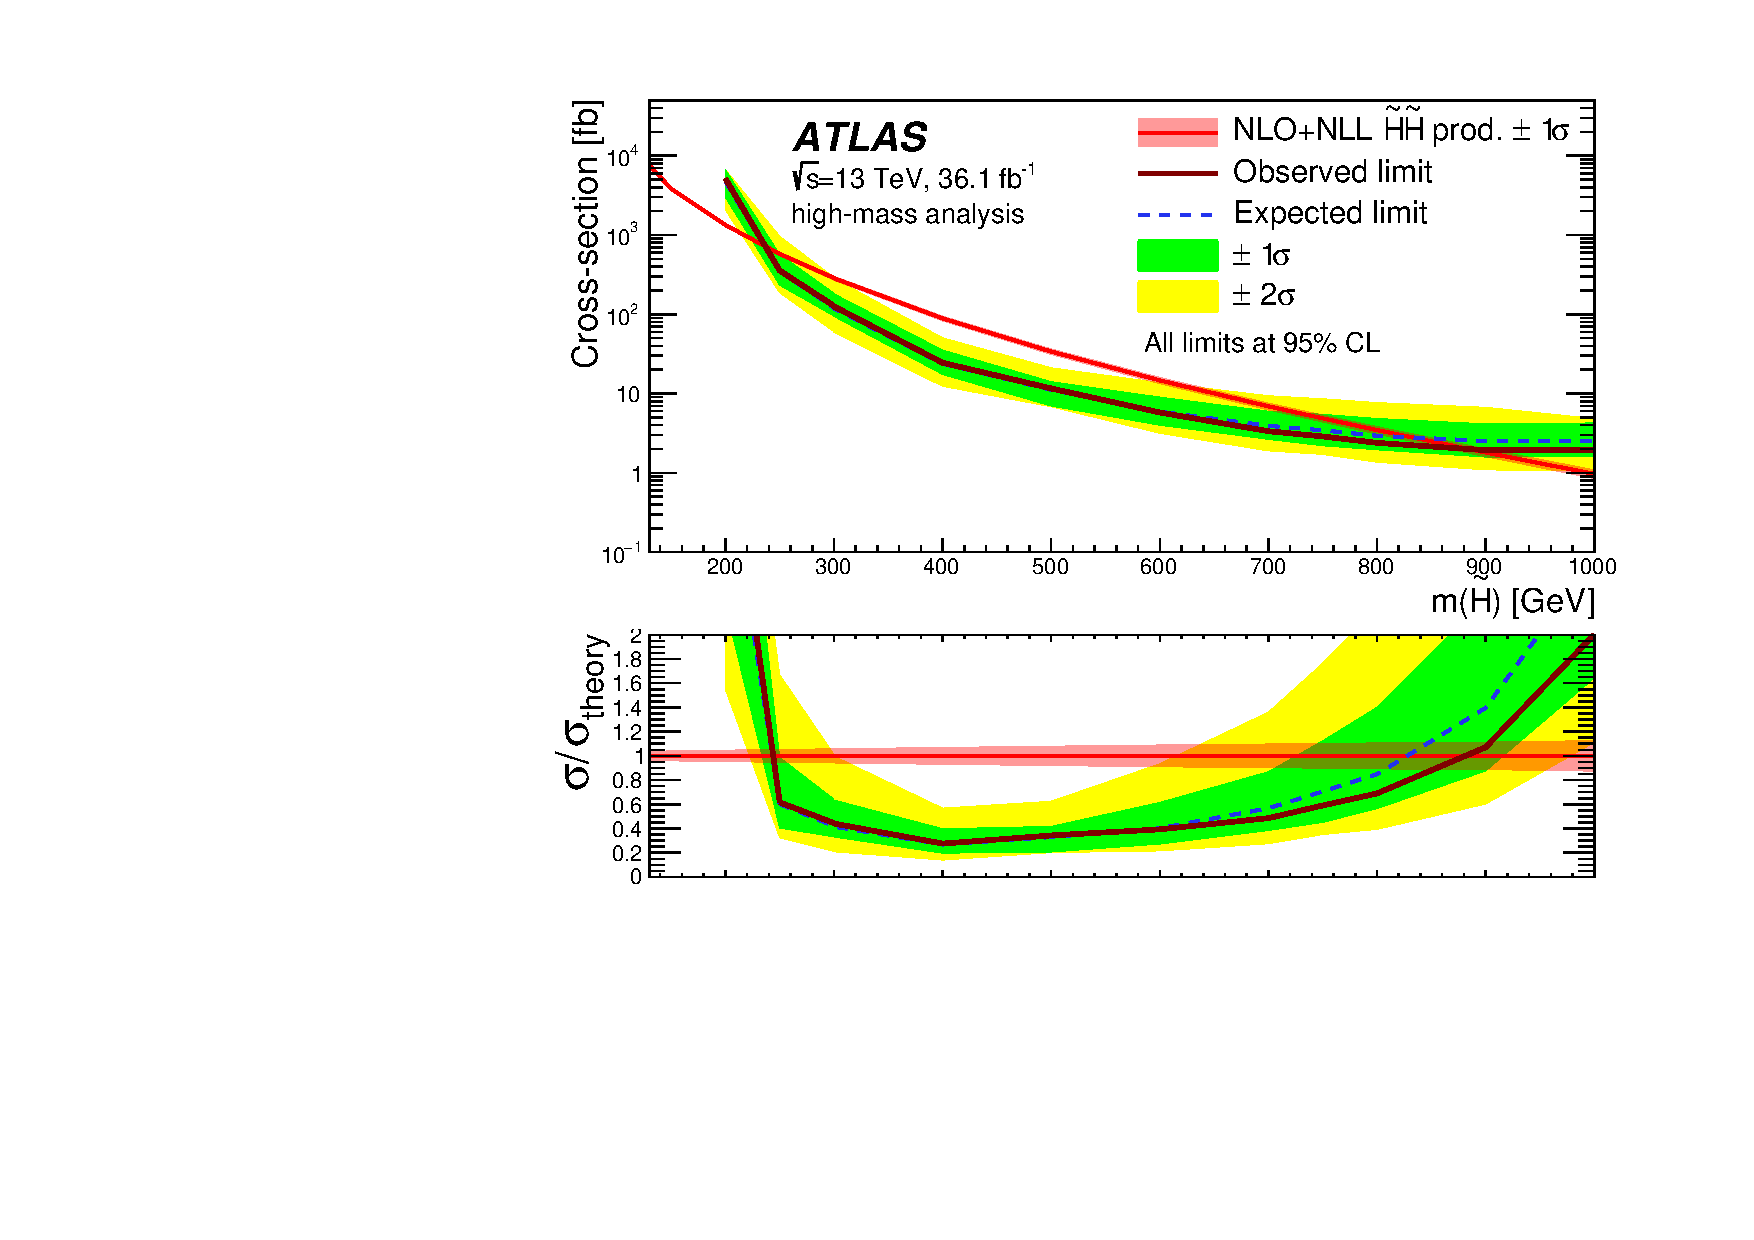
\includegraphics[width=0.8\textwidth]{figures/ewk_prod/interpretation/limit_HM}
	\caption{The observed (solid black) vs expected (dashed black) 95\% upper limits on the total pair production cross-section for degenerate higgsinos as a function of \mhino. The 1$\sigma$ and 2$\sigma$ uncertainty bands are shown as green and yellow, respectively. The theory cross-section is shown in the red curve. The bottom panel shows the ratio of the observed and expected limits with the theory cross-section. Figure from Ref. \cite{Aaboud:2018htj}.} 
	\label{fig:exclusion_high}
\end{figure}

\begin{figure}[htbp]
	\centering
	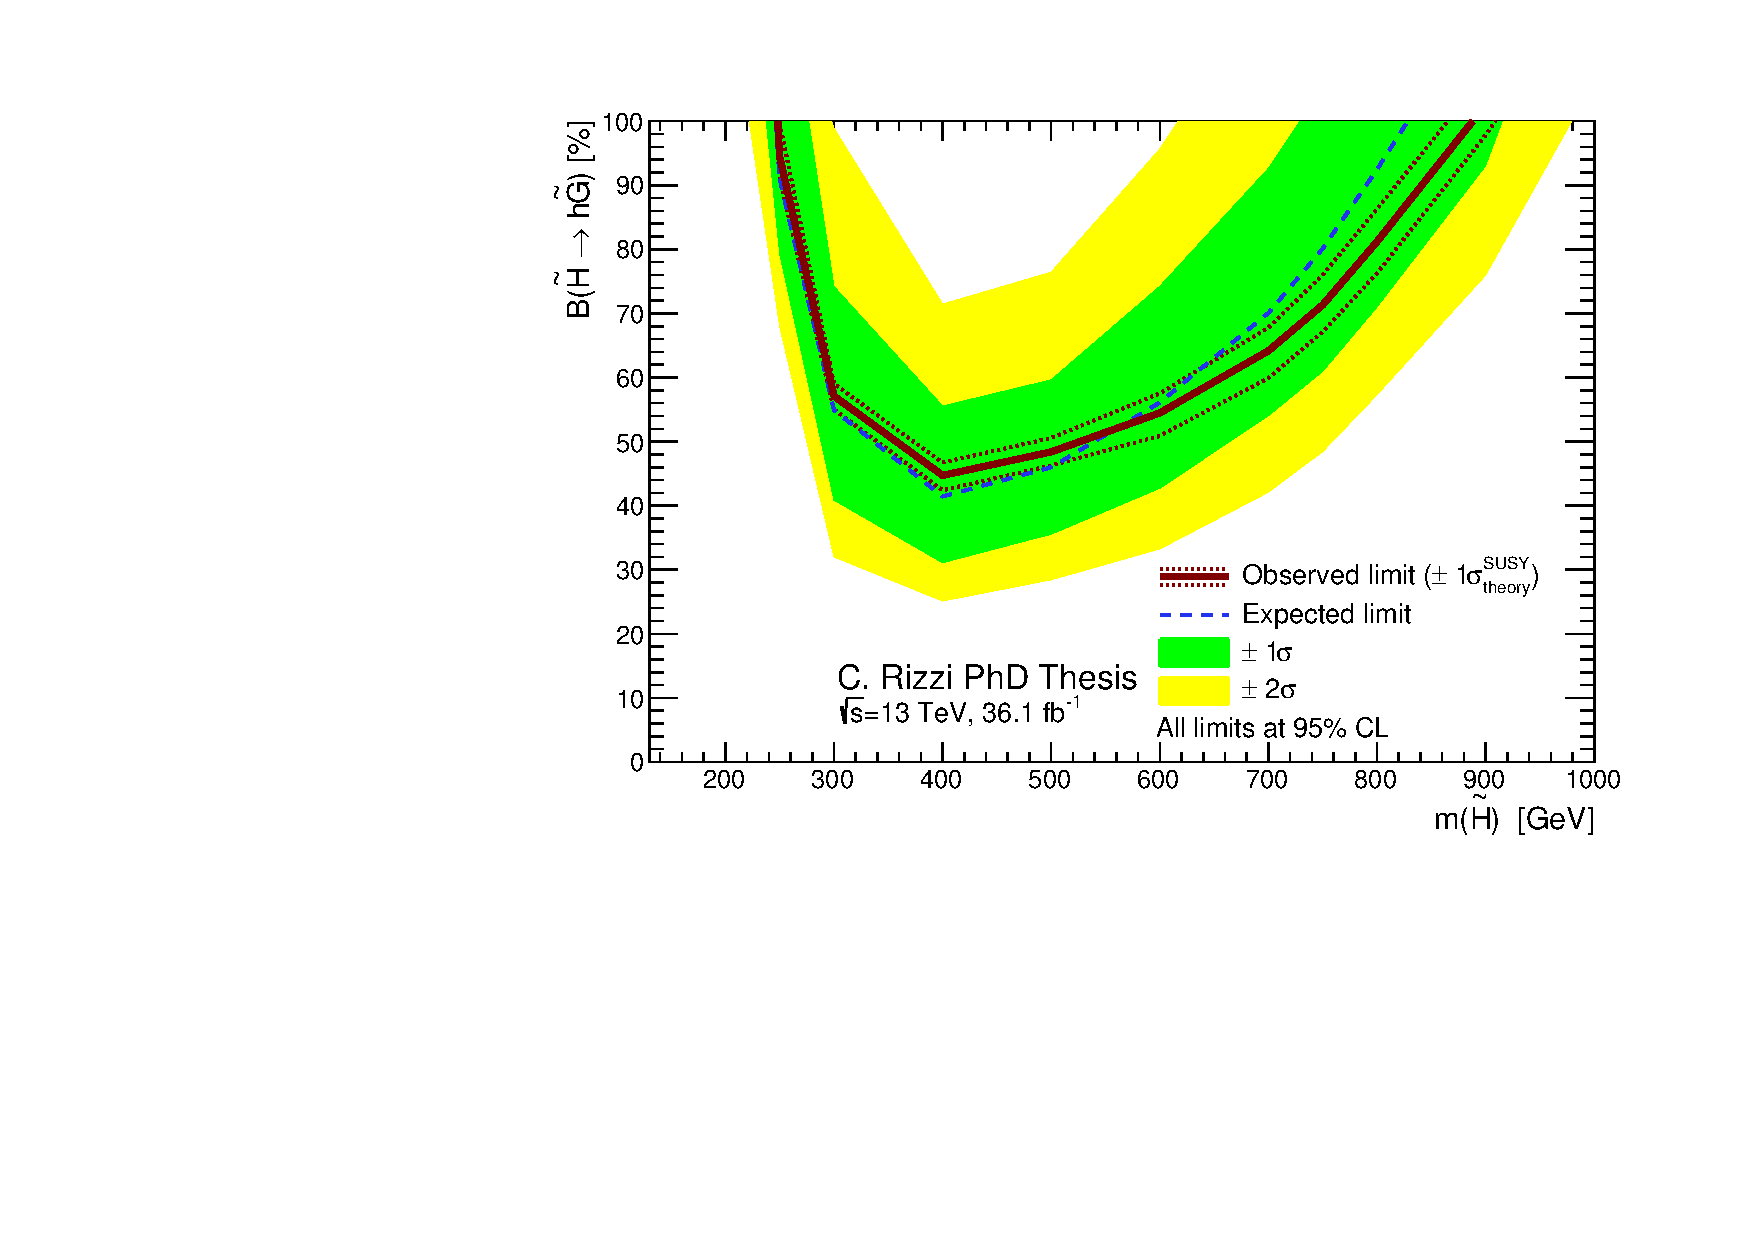
\includegraphics[width=0.8\textwidth]{figures/ewk_prod/interpretation/br_limit_HM.pdf}
	\caption{The observed (solid) vs expected (dashed) 95\% limits in the \mhino--\gls{br}$(\hino\rightarrow h \tilde{G})$ plane, where \gls{br}$(\hino\rightarrow h \tilde{G})$ denotes the branching ratio for the decay $\hino \rightarrow h \gravino$. The 1$\sigma$ uncertainty band is overlaid in green and the 2$\sigma$ in yellow. The regions above the lines are excluded by the analysis.} 
	\label{fig:exclusion_high:BR}
\end{figure}

\FloatBarrier

